%% Creator: Inkscape inkscape 0.92.5, www.inkscape.org
%% PDF/EPS/PS + LaTeX output extension by Johan Engelen, 2010
%% Accompanies image file 'layout_vib.pdf' (pdf, eps, ps)
%%
%% To include the image in your LaTeX document, write
%%   \input{<filename>.pdf_tex}
%%  instead of
%%   \includegraphics{<filename>.pdf}
%% To scale the image, write
%%   \def\svgwidth{<desired width>}
%%   \input{<filename>.pdf_tex}
%%  instead of
%%   \includegraphics[width=<desired width>]{<filename>.pdf}
%%
%% Images with a different path to the parent latex file can
%% be accessed with the `import' package (which may need to be
%% installed) using
%%   \usepackage{import}
%% in the preamble, and then including the image with
%%   \import{<path to file>}{<filename>.pdf_tex}
%% Alternatively, one can specify
%%   \graphicspath{{<path to file>/}}
%% 
%% For more information, please see info/svg-inkscape on CTAN:
%%   http://tug.ctan.org/tex-archive/info/svg-inkscape
%%
\begingroup%
  \makeatletter%
  \providecommand\color[2][]{%
    \errmessage{(Inkscape) Color is used for the text in Inkscape, but the package 'color.sty' is not loaded}%
    \renewcommand\color[2][]{}%
  }%
  \providecommand\transparent[1]{%
    \errmessage{(Inkscape) Transparency is used (non-zero) for the text in Inkscape, but the package 'transparent.sty' is not loaded}%
    \renewcommand\transparent[1]{}%
  }%
  \providecommand\rotatebox[2]{#2}%
  \newcommand*\fsize{\dimexpr\f@size pt\relax}%
  \newcommand*\lineheight[1]{\fontsize{\fsize}{#1\fsize}\selectfont}%
  \ifx\svgwidth\undefined%
    \setlength{\unitlength}{5cm}%
    \ifx\svgscale\undefined%
      \relax%
    \else%
      \setlength{\unitlength}{\unitlength * \real{\svgscale}}%
    \fi%
  \else%
    \setlength{\unitlength}{\svgwidth}%
  \fi%
  \global\let\svgwidth\undefined%
  \global\let\svgscale\undefined%
  \makeatother%
  \begin{picture}(1,1.76456311)%
    \lineheight{1}%
    \setlength\tabcolsep{0pt}%
    \put(0,0){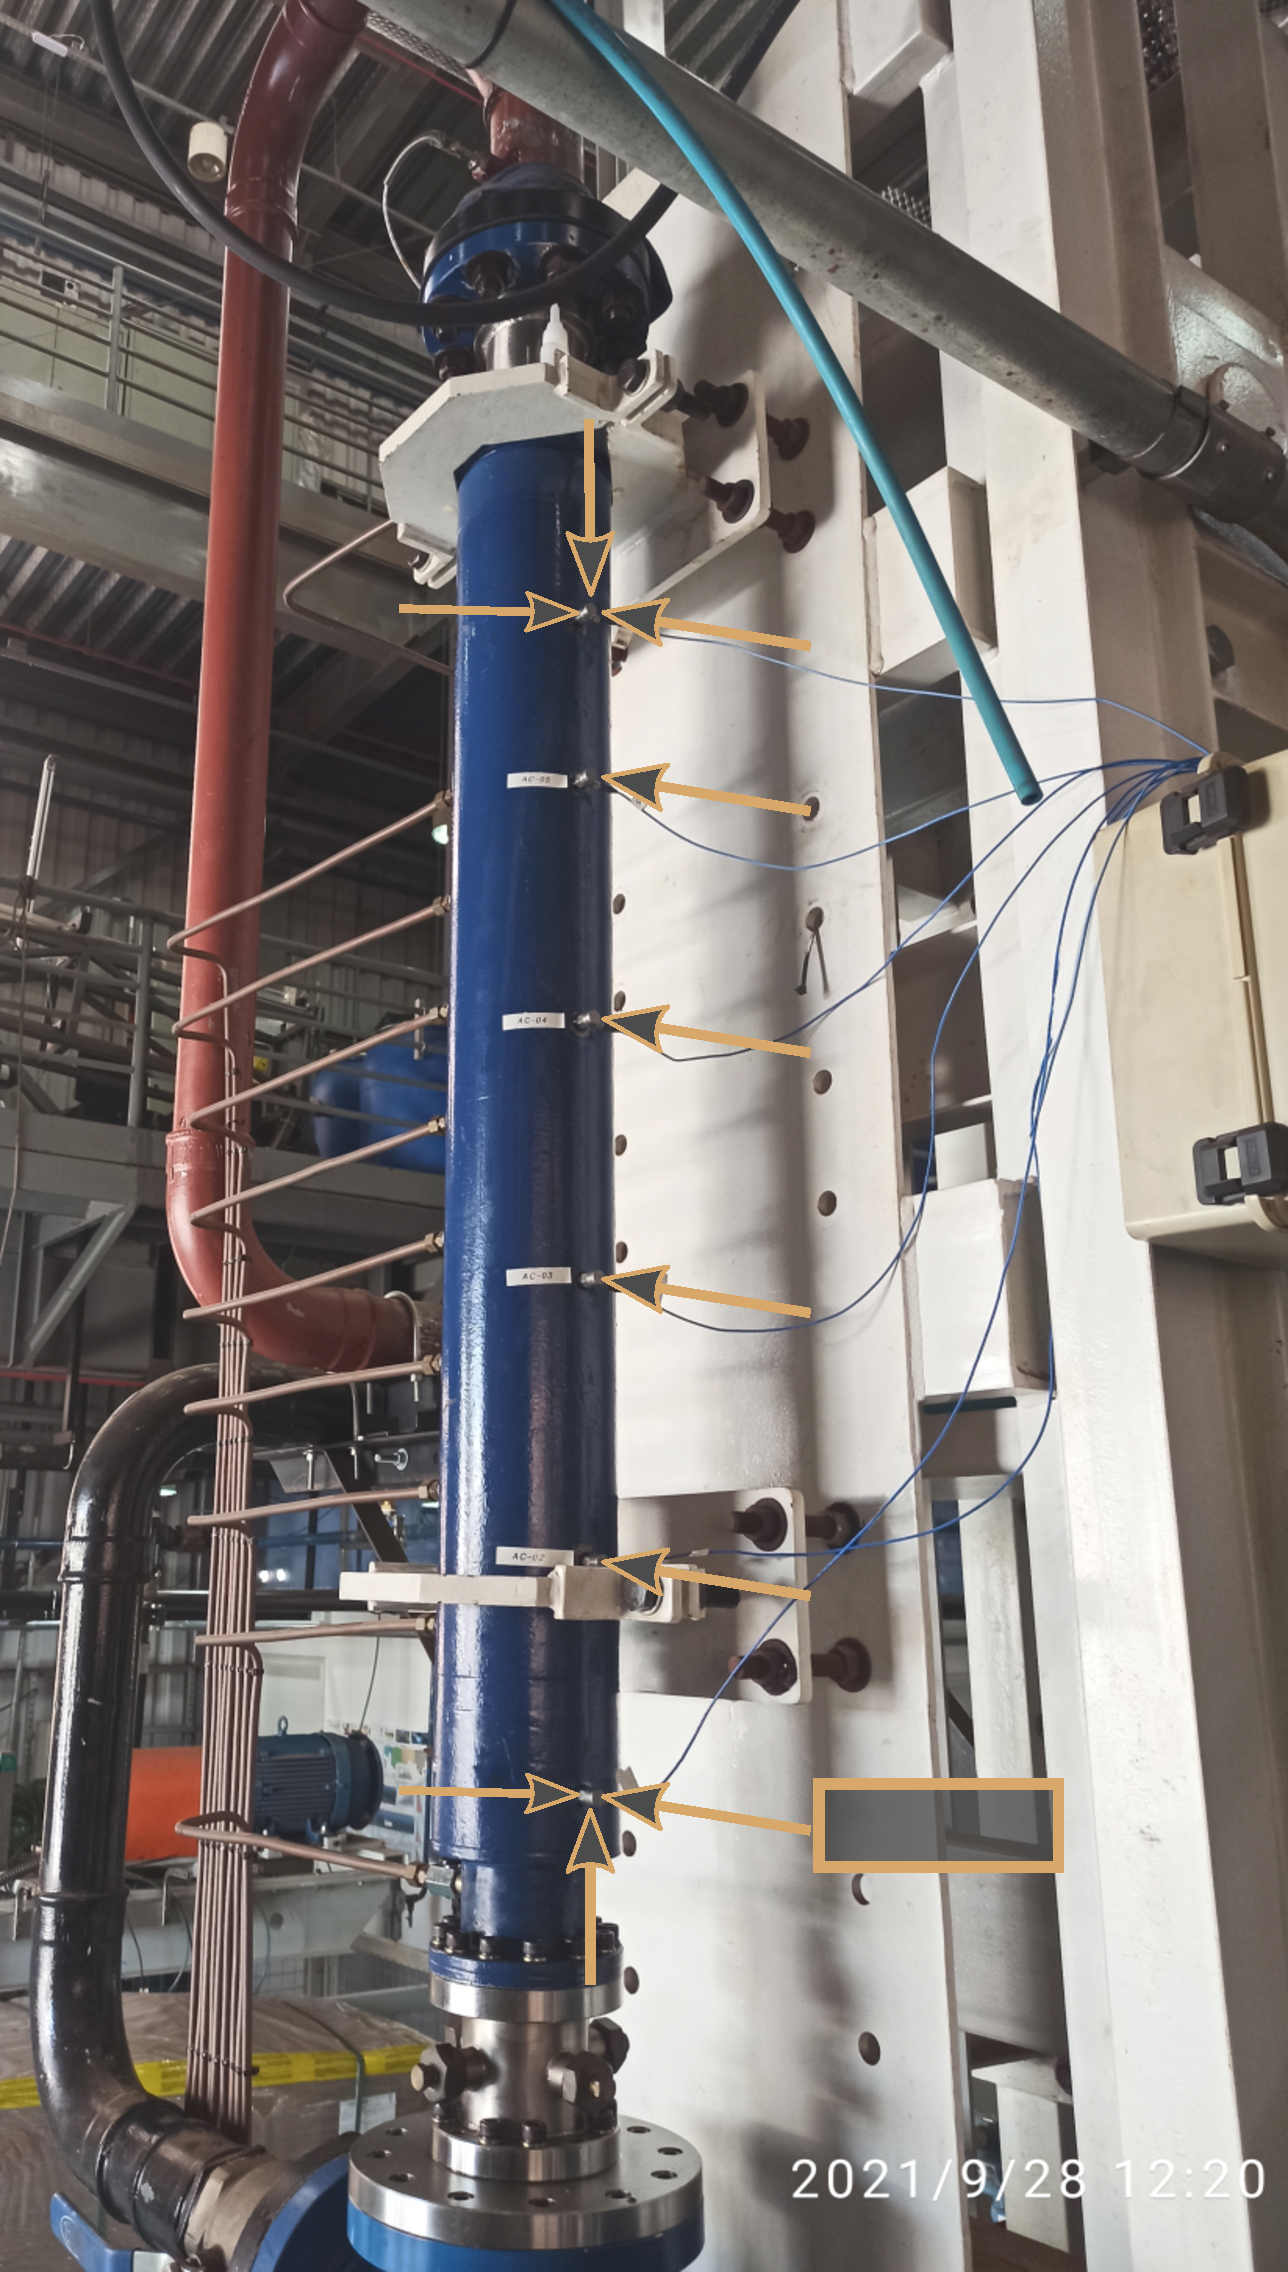
\includegraphics[width=\unitlength,page=1]{layout_vib.pdf}}%
    \put(0.65806877,0.33265345){\color[rgb]{0.84705882,0.65882353,0.41960784}\transparent{0.98000002}\makebox(0,0)[lt]{\lineheight{1.25}\smash{\begin{tabular}[t]{l} \tiny AC-01X\end{tabular}}}}%
    \put(0,0){\includegraphics[width=\unitlength,page=2]{layout_vib.pdf}}%
    \put(0.67270777,0.51639141){\color[rgb]{0.84705882,0.65882353,0.41960784}\transparent{0.98000002}\makebox(0,0)[lt]{\lineheight{1.25}\smash{\begin{tabular}[t]{l} \tiny AC-02\end{tabular}}}}%
    \put(0,0){\includegraphics[width=\unitlength,page=3]{layout_vib.pdf}}%
    \put(0.67270777,0.73557861){\color[rgb]{0.84705882,0.65882353,0.41960784}\transparent{0.98000002}\makebox(0,0)[lt]{\lineheight{1.25}\smash{\begin{tabular}[t]{l} \tiny AC-03\end{tabular}}}}%
    \put(0,0){\includegraphics[width=\unitlength,page=4]{layout_vib.pdf}}%
    \put(0.67270777,0.92605636){\color[rgb]{0.84705882,0.65882353,0.41960784}\transparent{0.98000002}\makebox(0,0)[lt]{\lineheight{1.25}\smash{\begin{tabular}[t]{l} \tiny AC-04\end{tabular}}}}%
    \put(0,0){\includegraphics[width=\unitlength,page=5]{layout_vib.pdf}}%
    \put(0.67270777,1.11643992){\color[rgb]{0.84705882,0.65882353,0.41960784}\transparent{0.98000002}\makebox(0,0)[lt]{\lineheight{1.25}\smash{\begin{tabular}[t]{l} \tiny AC-05\end{tabular}}}}%
    \put(0,0){\includegraphics[width=\unitlength,page=6]{layout_vib.pdf}}%
    \put(0.65806877,1.27749431){\color[rgb]{0.84705882,0.65882353,0.41960784}\transparent{0.98000002}\makebox(0,0)[lt]{\lineheight{1.25}\smash{\begin{tabular}[t]{l} \tiny AC-06X\end{tabular}}}}%
    \put(0,0){\includegraphics[width=\unitlength,page=7]{layout_vib.pdf}}%
    \put(0.16350434,0.41449444){\color[rgb]{0.84705882,0.65882353,0.41960784}\transparent{0.98000002}\makebox(0,0)[lt]{\lineheight{1.25}\smash{\begin{tabular}[t]{l} \tiny AC-01Y\end{tabular}}}}%
    \put(0,0){\includegraphics[width=\unitlength,page=8]{layout_vib.pdf}}%
    \put(0.50315522,0.23519379){\color[rgb]{0.84705882,0.65882353,0.41960784}\transparent{0.98000002}\makebox(0,0)[lt]{\lineheight{1.25}\smash{\begin{tabular}[t]{l} \tiny AC-01Z\end{tabular}}}}%
    \put(0,0){\includegraphics[width=\unitlength,page=9]{layout_vib.pdf}}%
    \put(0.50315522,1.39153084){\color[rgb]{0.84705882,0.65882353,0.41960784}\transparent{0.98000002}\makebox(0,0)[lt]{\lineheight{1.25}\smash{\begin{tabular}[t]{l} \tiny AC-06Z\end{tabular}}}}%
    \put(0,0){\includegraphics[width=\unitlength,page=10]{layout_vib.pdf}}%
    \put(0.16350434,1.21749675){\color[rgb]{0.84705882,0.65882353,0.41960784}\transparent{0.98000002}\makebox(0,0)[lt]{\lineheight{1.25}\smash{\begin{tabular}[t]{l} \tiny AC-06Y\end{tabular}}}}%
    \put(0,0){\includegraphics[width=\unitlength,page=11]{layout_vib.pdf}}%
    \put(0.25 ,0.27){\color[rgb]{1,1,1}\makebox(0,0)[lt]{\lineheight{1.25}\smash{\begin{tabular}[t]{l} \tiny {$P_1$}\end{tabular}}}}%
    \put(0,0){\includegraphics[width=\unitlength,page=12]{layout_vib.pdf}}%
    \put(0.25 ,1.14){\color[rgb]{1,1,1}\makebox(0,0)[lt]{\lineheight{1.25}\smash{\begin{tabular}[t]{l} \tiny {$P_9$}\end{tabular}}}}%
    \put(0,0){\includegraphics[width=\unitlength,page=13]{layout_vib.pdf}}%
    \put(0.508,0.164){\color[rgb]{1,1,1}\makebox(0,0)[lt]{\lineheight{1.25}\smash{\begin{tabular}[t]{l} \tiny {$T_2$}\end{tabular}}}}%
    \put(0,0){\includegraphics[width=\unitlength,page=14]{layout_vib.pdf}}%
    \put(0.45841374,1.632){\color[rgb]{1,1,1}\makebox(0,0)[lt]{\lineheight{1.25}\smash{\begin{tabular}[t]{l} \tiny {$T_3$}\end{tabular}}}}%
  \end{picture}%
\endgroup%
